\section{Zweidimensionales Punktediagramm}

Da das zweidimensionale Punktediagramm weit verbreitet ist, sind sich Betrachter an diese Darstellung gewöhnt. Oft werden die Punkte in Diagramm durch eine Linie verbunden, was den Verlauf der abgebildeten Datenwerte verdeutlicht, besonders in Medien, zum Bespiel für die Darstellung von Börsenkursen. 

Aus diesem Grund wurde als erstes Beispiel das zweidimensionale Punktediagramm (beziehungsweise das Liniendiagramm, falls Linien hinzugefügt werden) ausgewählt.

\subsection{Information-Seeking Mantra}

Als Startreferenz für die Entwicklung des interaktiven Diagrammes bieten sich die von Ben Shneiderman begründeten Prinzipien für das Design graphischer Benutzeroberflächen an, das "`\textit{Information-Seeking Mantra}"'. Die Weise, wie der Benutzer mit der Oberfläche interagiert, hat Shneiderman \cite{shneiderman} festgelegt:

\begin{itemize}
	\item Überblick ("`\textit{Overview first}"')
	\item Zoomen und Filtern ("`\textit{zoom and filter}"')
	\item Details auf Abruf ("`\textit{then details-on-demand}"')
\end{itemize}

\textbf{Überblick.} Der Benutzer verschafft sich einen Überblick über die gesamte Oberfläche des Programms.

\textbf{Zoom.} Zur besseren Betrachtung vergrössert der Benutzer die Ansicht, sodass die betreffenden Elemente grösser angezeigt werden.

\textbf{Filter.} Die Filter-Funktion ermöglicht dem Benutzer, gewisse Elemente oder Elementgruppen je nach Interesse ein- oder auszublenden.

\textbf{Details auf Abruf.} Falls ein Element den Nutzer besonders interessiert, besteht die Möglichkeit, dass zusätzliche relevante Informationen zum Element angezeigt werden können.

Zusätzlich formulierte Shneiderman drei weitere Schritte:

\textbf{Zusammenhänge betrachten.} Die Zusammenhänge zwischen den verschiedenen Elementen können im Programm betrachtet werden. Diesen Schritt umzusetzen ist nur bei wenigen Benutzeroberflächen sinnvoll, zum Beispiel bei der Darstellung von Baumdiagrammen oder anderen Diagramme mit hierarchischen Daten.

\textbf{Verlauf.} Die Interaktionen des Benutzers mit der Programmoberfläche werden aufgezeichnet. Dadurch können Interaktionen rückgängig gemacht werden.

\textbf{Extraktion.} Damit wird die Extraktion erlaubt der \textit{Query-Parameter} (wie angewandte Filter, Verlauf, Zoomstufe) und der durch die Interaktion bereits definierten Elementgruppen ("`\textit{subcollections}"').

Im Diagramm werden nur die Methoden \textit{Überblick}, \textit{Zoom}, \textit{Filter} und \textit{Details auf Abruf} umgesetzt. Das Mantra wurde allgemein für Benutzeroberflächen von Programmen beschrieben, in unserer Applikation, einem interaktiven Diagramm, macht aber die Umsetzung der Schritte \textit{Zusammenhänge betrachten}, \textit{Verlauf}, \textit{Extraktion} in Bezug auf die Funktion des Diagramms keinen Sinn:

\begin{itemize}
	\item Punktediagramme oder Liniendiagramme werden nicht dazu verwendet, Daten in Hierarchieform darzustellen.
	\item Die Interaktionen im Diagramm sind zu banal, als dass eine Rückgängig-Funktion von Nutzen wäre.
	\item Die Extraktion und der Export von Query-Parametern des Diagramms ist zwar theoretisch umzusetzen, ist jedoch von minimaler praktischer Bedeutung.
	\item Zur Extraktion von "`\textit{subcollections}"' aus einem Datensatz sollte kein interaktives Diagramm verwendet werden. Eine Datenverarbeitungsapplikation ist für diese Aufgabe angemessener, da exakte Parameter zur Extraktion bestimmt werden können.
\end{itemize}

\newpage

\subsection{Applikation}

\begin{figure}[!htbp]
	\centering
	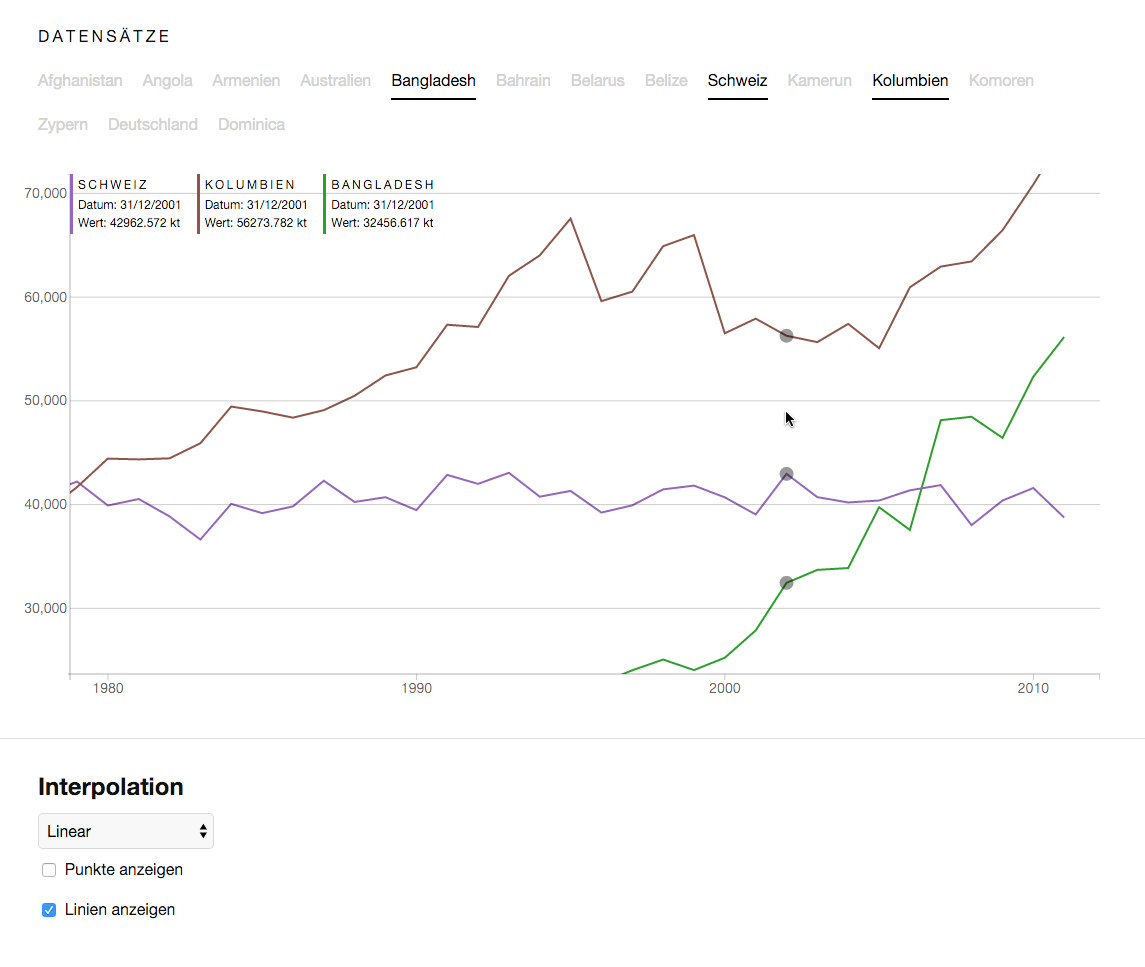
\includegraphics[width=\linewidth]{images/2dline}
	\caption{Screenshot der Oberfläche der Applikation (zweidimensionales Liniendiagramm / Punktediagramm)}
	\label{fig:scatterplot}
\end{figure}

% TODO fuckin bullet points please bith